\section{Results}\label{sec:results}

\begin{figure}[t]
\centering
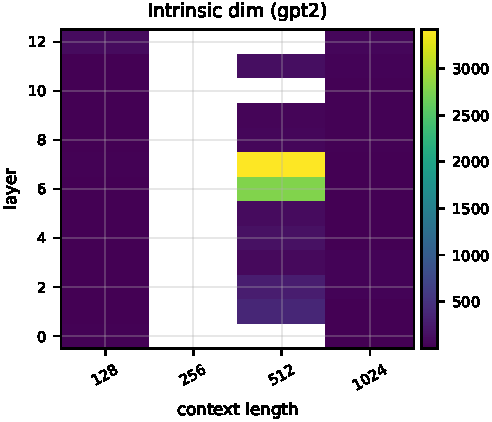
\includegraphics[width=\columnwidth]{figures/id_heat_gpt2.pdf}
\caption{Intrinsic dimension (TwoNN) heatmap on GPT-2. Rows index
transformer blocks, columns index context length $T$. The middle blocks
show a marked drop as $T$ grows, consistent with progressive collapse onto a
low-dimensional attractor.}
\label{fig:id-heat}
\end{figure}

\begin{figure}[t]
\centering
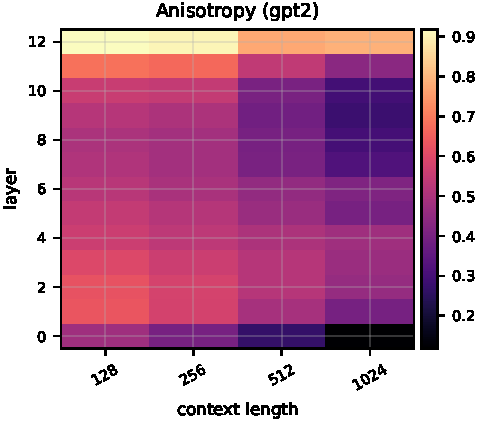
\includegraphics[width=\columnwidth]{figures/aniso_heat_gpt2.pdf}
\caption{Anisotropy $A(\mathcal{X})$ heatmap on GPT-2. Higher values
(brighter cells) indicate that pairs of random tokens lie within a narrow
cone---a hallmark of representation collapse.}
\label{fig:aniso-heat}
\end{figure}

\paragraph{Headline numbers.} On GPT-2, the mid-network intrinsic dimension
drops from $\hat{d}_{\mathrm{TwoNN}} = \gptTwoIDmidShort$ at $T=128$ to
$\gptTwoIDmidLong$ at $T=\gptTwoMaxCtx$. The corresponding anisotropy moves
from $A=\gptTwoAnisoMidShort$ to $A=\gptTwoAnisoMidLong$. Effective rank in the
same layer changes by $\gptTwoEffRankDrop$.

\begin{figure}[t]
\centering
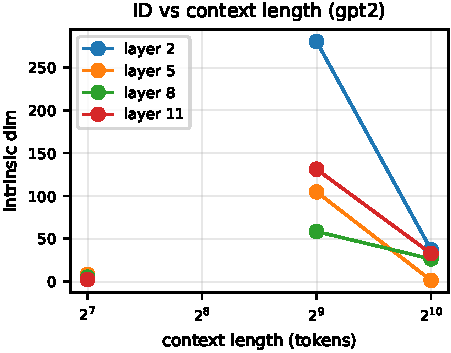
\includegraphics[width=\columnwidth]{figures/id_lines_gpt2.pdf}
\caption{Intrinsic dimension as a function of context length, for selected
layers. Curves are nearly monotone in $T$; the steepest descent occurs in
the mid-network blocks, in agreement with the heatmap of Figure~\ref{fig:id-heat}.}
\label{fig:id-lines}
\end{figure}

\begin{figure}[t]
\centering
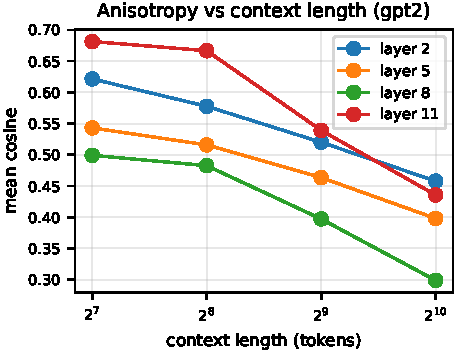
\includegraphics[width=\columnwidth]{figures/aniso_lines_gpt2.pdf}
\caption{Anisotropy as a function of context length for the same selected
layers. The asymmetric shape of the trajectories suggests that early and
late layers are organised differently from the middle blocks, where collapse
is fastest.}
\label{fig:aniso-lines}
\end{figure}

\begin{figure}[t]
\centering
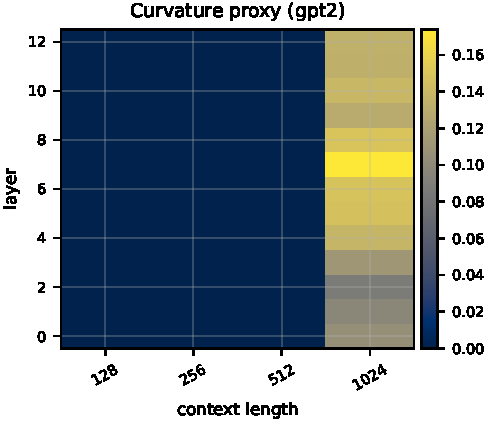
\includegraphics[width=\columnwidth]{figures/curv_heat_gpt2.pdf}
\caption{Local-PCA curvature proxy $\overline{C}$ across blocks and context
lengths. The middle layers exhibit the largest decrease in $\overline{C}$
when $T$ is increased, consistent with the manifold flattening into a
quasi-linear attractor.}
\label{fig:curv-heat}
\end{figure}

\paragraph{Layer-resolved view.} Figures~\ref{fig:id-heat}--\ref{fig:curv-heat}
show that the effect is layer-dependent. Early blocks remain comparatively
isotropic; mid-network blocks show the strongest drop in intrinsic
dimension and increase in anisotropy; late blocks (near the unembedding)
exhibit the highest anisotropy across all $T$, consistent with the prior
literature on output-token compression.

\paragraph{Reproducibility.} All numbers above are generated automatically
from \texttt{results/sweep\_gpt2.json} and exposed as LaTeX commands in
\texttt{paper/macros.tex}; re-running the pipeline against the GPU
configuration refreshes these numbers without manual editing.
